\chapter{Marshaling between C\# and C Part 2}
\section{String Marshaling}
For this part, we'll need to create a dotnet core console project for Chapter 6 and make sure to reference ''AdvancedDLSupport'' on nuget. You will need to add a build task for this project to compile C code after building C\# code. Your CSProj file should have the following:
\lstinputlisting[style=customxml, language=XML]{codes/Chap6/Chap6Snippet1.xml}

Over the course of this lesson, we'll go over the differences between By Value String and C Ansi String (char*). It important to keep in mind that in C\#, string is a reference type and is an immutable type as well meaning, the content of the string shouldn't be modified during runtime and in that case, we would use StringBuilder which can be used for this situation (we can specify the capacity for initial size of StringBuilder.) The marshaling will marshal the reference to content of string to C native code and back almost seamlessly.

\newpage
And for this lesson, we will have a few functions to play with for string manipulation from C Library:

\lstinputlisting[style=customc, language=C]{codes/Chap6/Chap6Snippet2.c}

As you may have noticed, we are attempting to marshal both C Ansi String and By Value String.
\newpage
\lstinputlisting[style=customcs]{codes/Chap6/Chap6Snippet3.cs}

And the output will be as followed:

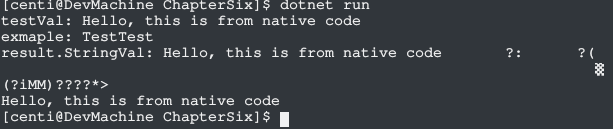
\includegraphics[width=\textwidth]{ChapSixConsole}
\newpage

There are few things happening here, the `testVal` line demonstrate the string builder with the capacity of 128 characters, but when running SetDefaultMessage2, the Marshaler will determine the size of string written to StringBuilder with either strlen or wcslen depending on the character set for SetDefaultMessage2 and have content of string copied over to StringBuilder. Due to the nature of strlen and wcslen, it will copy the string up to null terminated character and you can test this by adding \textbackslash 0 in DefaultMsg string in C source file and P/Invoke Marshaler will null terminated the string copying.

The `example:` line demonstrate that StringBuilder will still print even with null terminated character in C\#, it does not terminate the string at the first null terminated character, this illustrate that the process seen in first line is purely done by P/Invoke Marshaling.

The `result.StringVal` line is a little more complex, but what is going on is that the ByValCharArray is quite literally a ValueType that store string data within it and it have a fixed size of 128 characters and when running SetDefaultMessage, it would print a string that includes null terminated characters and other data that aren't zeroed out when allocated, P/Invoke Marshaler have no process or handle on how this data is copied, this is useful if this the intended behavior you desire.

The last line demonstrate the print of null terminated string that is read from third line.

The ValueType char array can be useful for recycling same data container without allocating/reallocating/disposing data in an iteration and thus enabling a more efficient code and less memory pressure on the process.


\section{Pointer Marshaling}

\section{Function Marshaling}